\documentclass{nature}
\usepackage{amsmath,amssymb,graphicx,hyperref} 

\usepackage{epsfig}
%\usepackage{showkeys}
\usepackage{subfigure}

\graphicspath{{Figures/}}


\title{Shocks and GW from PBH formation}


\author{Ue-Li Pen, Neil Turok}
%\email{pen@cita.utoronto.ca}
\begin{document}
\maketitle

\begin{affiliations}
\footnotesize{
\item {Canadian Institute of Theoretical Astrophysics, 60 St George St, Toronto, ON M5S 3H8, Canada.}
\item {Canadian Institute for Advanced Research, CIFAR program
  in Gravitation and Cosmology.}
\item {Dunlap Institute for Astronomy \& Astrophysics, University of Toronto, AB 120-50 St. George Street, Toronto, ON M5S 3H4, Canada.}
\item {Perimeter Institute of Theoretical Physics, 31 Caroline Street North, Waterloo, ON N2L 2Y5, Canada.}
}
\end{affiliations}

\begin{abstract}
We discuss gravitational waves signature from primordial black hole formation.
\end{abstract}


\section{Introduction and Summary}

Recently \cite{2016arXiv160300464B} proposed that the recent LIGO
detections\cite{2016PhRvL.116f1102A,2016PhRvL.116x1103A} could be due
to mergers of primordial black holes.  In this letter we examine the
acoustic waves generated during this process, and show that they
generically lead to gravitational waves through two processes: second
order wave interactions and shock formation, which cascades the power
from the horizon scale down to the neutrino diffusion scale, leading
to gravitational waves detectable by advanced LIGO.

\section{Length Scales}

The earliest plausible time to causally form black holes of $M\sim$
thirty solar masses is when the horizon size contains $M$.  About
$10^{-9}$ of the radiation density would need to form black holes.  We
consider two types of sources for fluctuations which lead to PBH.
Firstly, an initial feature in the power spectra at this scale with an
amplitude of $\sim 20\%$ would lead to collapse of a comparable mass
fraction into PBHs\cite{Kühnel2016}.  Secondly, if the QCD phase
transition were first order, rare bubbles could also lead to PBHs.  In
either scenario, regions which did not form black holes would
nevertheless generate sound waves.  Two different mechanisms are
understood by which these sound waves will generate shock waves.  At
second order in perturbation theory, these will generate large
amplitudes of gravitational waves in the $\mu$Hz
band\cite{2007PhRvD..76h4019B}, which may be detectable by space based
interferometers\footnote{https://www.elisascience.org}.  The amplitude
of these waves would be $h \sim 10^{-14}$, which may be accessible to
future pulsar timing arrays\cite{kramer04}.

As recently shown\cite{2015arXiv151002985P}, these sound waves will
steepen into shock waves with thin transition regions given by the
neutrino diffusion length\cite{2014PhRvL.113f1301J}.  These shock
waves will source gravitational waves at a wide range of frequencies,
with an amplitude $h\sim$, below current upper
bounds\cite{2015PhRvD..91b2003A}, but which could in turn be detected
by advanced LIGO.

\section{Stochastic gravitational wave background}
\begin{figure} \centering
  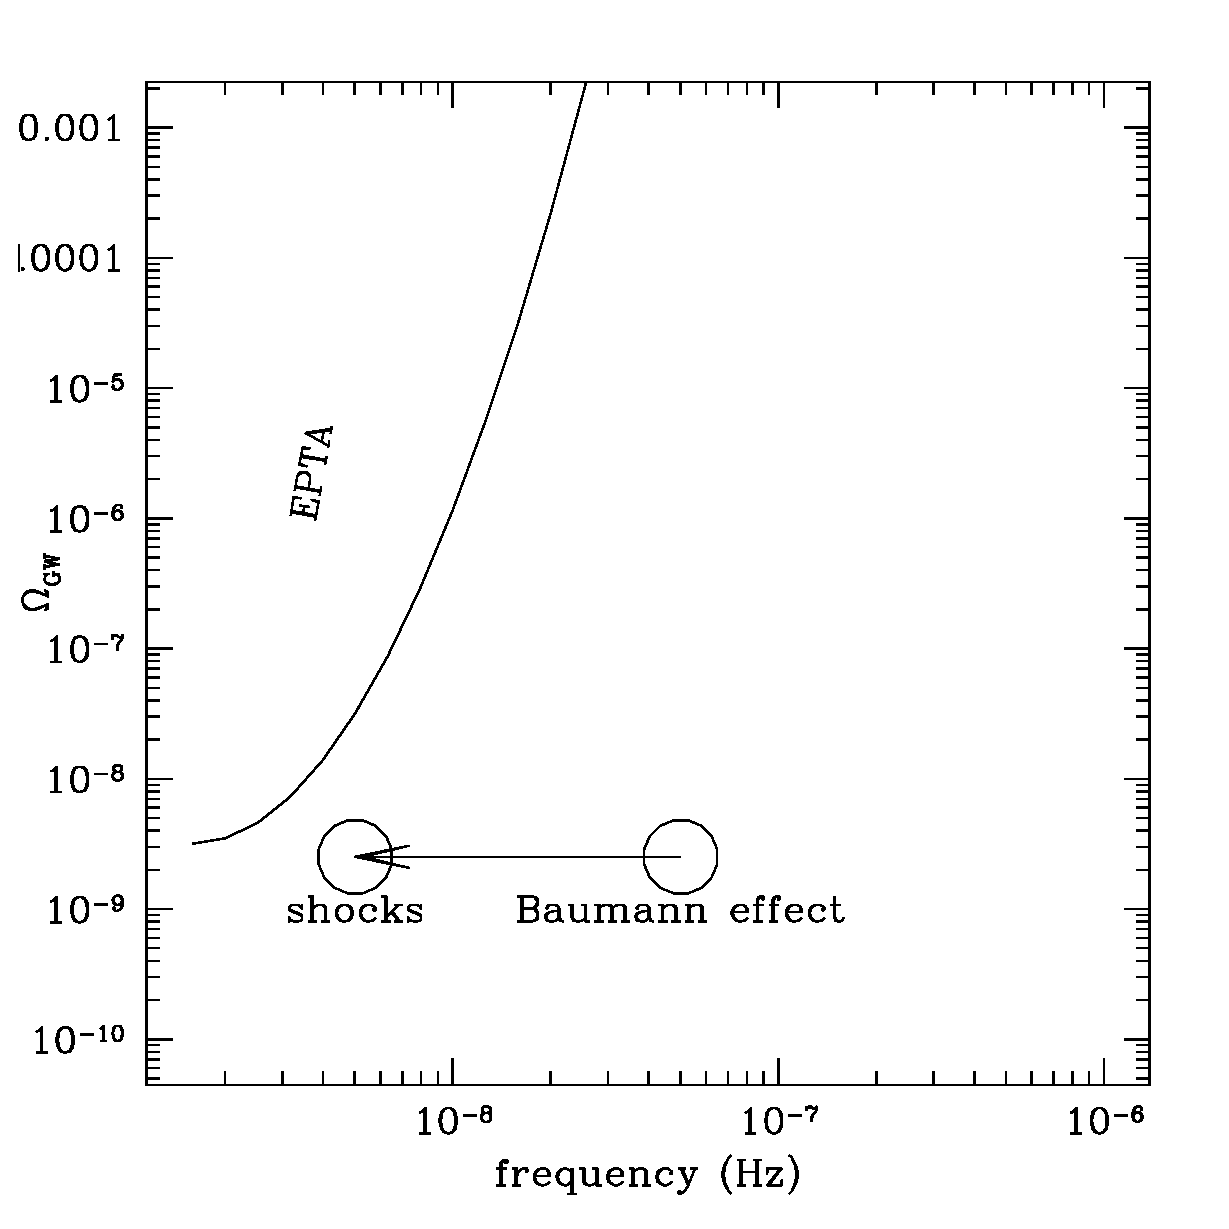
\includegraphics[width=1.0\linewidth]{gw.eps}
  \caption{\textbf{GW background.}
}
  \label{fig:gw}
\end{figure}

\section{Astronomical constraints}

Various astronomical constraints have been
proposed\cite{2016arXiv160706077C}. Most of these constraints are
entangled in astrophysical uncertainties, including for example black
hole accretion efficiencies, and baryonic feedback.  Gravitational
waves are a physically clean and inevitable product of the formation
process.



\begin{addendum}
\item 
This work is supported by the Canadian Government through the Canadian
Institute for Advance Research and Industry Canada, and by Province of
Ontario through the Ministry of Research and Innovation.
\end{addendum}

\appendix

%\bibliographystyle{utcaps}
\bibliographystyle{naturemag}
\bibliography{pbh}


\end{document}
